\documentclass{ximera}

\title{The Idea of Limits}

\begin{document}
\begin{abstract}
This is a trial online lesson on an introduction to limits.
\end{abstract}
\maketitle

\section{Goals of this Lesson}
\subsection{Conceptual Goals:}

\begin{itemize}
\item Average velocity vs instaneous velocity
\item Secant live vs tangent line
\item What is a limit?
\end{itemize}

\subsection{Computational Goals:}

\begin{itemize}
\item Compute average velocity
\item Approximate instantaneous velocity
\item Calculus slope of a secant line
\end{itemize}


\section{Average Velocity}

\youtube{HwzVyIaiKcQ?autoplay=0&rel=0&end=97}

\begin{question}
  To find the average velocity over an interval, we should divide which two quantities?
  \begin{selectAll}
    \choice{The time when the interval ended}
    \choice{The final position of the ball}
    \choice[correct]{The length of time the interval lasted}
    \choice[correct]{The distance the ball traveled over the interval}
    \choice{The final speed of the ball}
    \choice{The intial position of the ball}
  \end{selectAll}
  \begin{feedback}
  The average velocity is the distance traveled divided by the length of the time interval.
  \end{feedback}
\end{question}

\begin{formula}
To find the average velocity:
\[
v_{av}=\frac{\text{change in position}}{\text{change in time}} = \frac{s(t_1)-s(t_0)}{t_1-t_0}
\]
where $s(t)$ is the position at time $t$ and the time interval $[t_0,t_1]$
\end{formula}

Practice Finding Average Velocity:
\begin{foldable}
\begin{image}
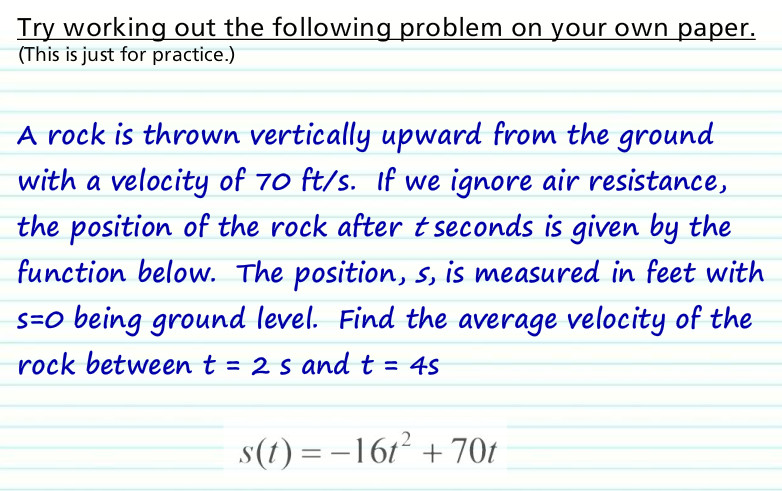
\includegraphics{picture1.jpg}
\end{image}
Click to see the solution:
\begin{foldable}
\begin{image}
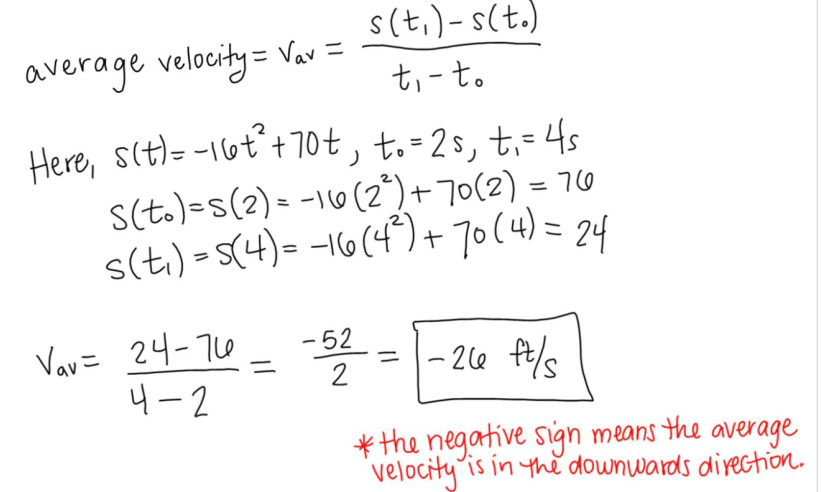
\includegraphics{picture2.jpg}
\end{image}
\end{foldable}

\end{foldable}
\end{document}
